%
\phantomsection
%\addcontentsline{toc}{chapter}{Implementation}
%
\chapter{Design and Implementation}
%
\markboth{Implementation}{Implementation}	% headings
%
\label{cap:implementation}
This chapter presents the design and implementation processes of the solution proposed by this work. The chapter will be divided in three main sections: Introduction, Dynamic Checkpoint Rate Tuning, Reliam Resource Allocation Policy.

In the {\hyperref[sec:introdes]{\emph{Introduction}}}, an overview on the general aim of the thesis and the framework in which it has been integrated will be provided. In Section {\hyperref[sec:dcrt]{\emph{Dynamic Checkpoint Rate Tuning}}}, the design and implementation of an innovative logic in the scheduling of the checkpointing routine will be explored. Finally, in {\hyperref[sec:reliam]{\emph{Reliam Resource Allocation Policy}}}, the design and implementation of our reliability aware resource allocation policy will be examined in depth.

\section{Introduction}
\label{sec:introdes}
As anticipated in {\hyperref[cap:introduction]{Chapter 1}}, technology scaling in the HPC landscape is contributing to making resource allocation policies of primary importance, as well as the need of a reliability manager able to guarantee a sensible usage of the processing elements at the available in the system. This work proposes a solution which proactively deals with the reliability issue both through a system-aware perspective, in order to tackle faults and aging of the hardware components, and through a application aware perspective, being able to adapt to the specific needs of the applications. RTRM and C/R tools, examined in {\hyperref[cap:stateofart]{Chapter 2}}, are exploited and shaped in order to fit the twofold purpose and reach the best reliability-performance trade off.

\begin{figure}[t]
    \centering
    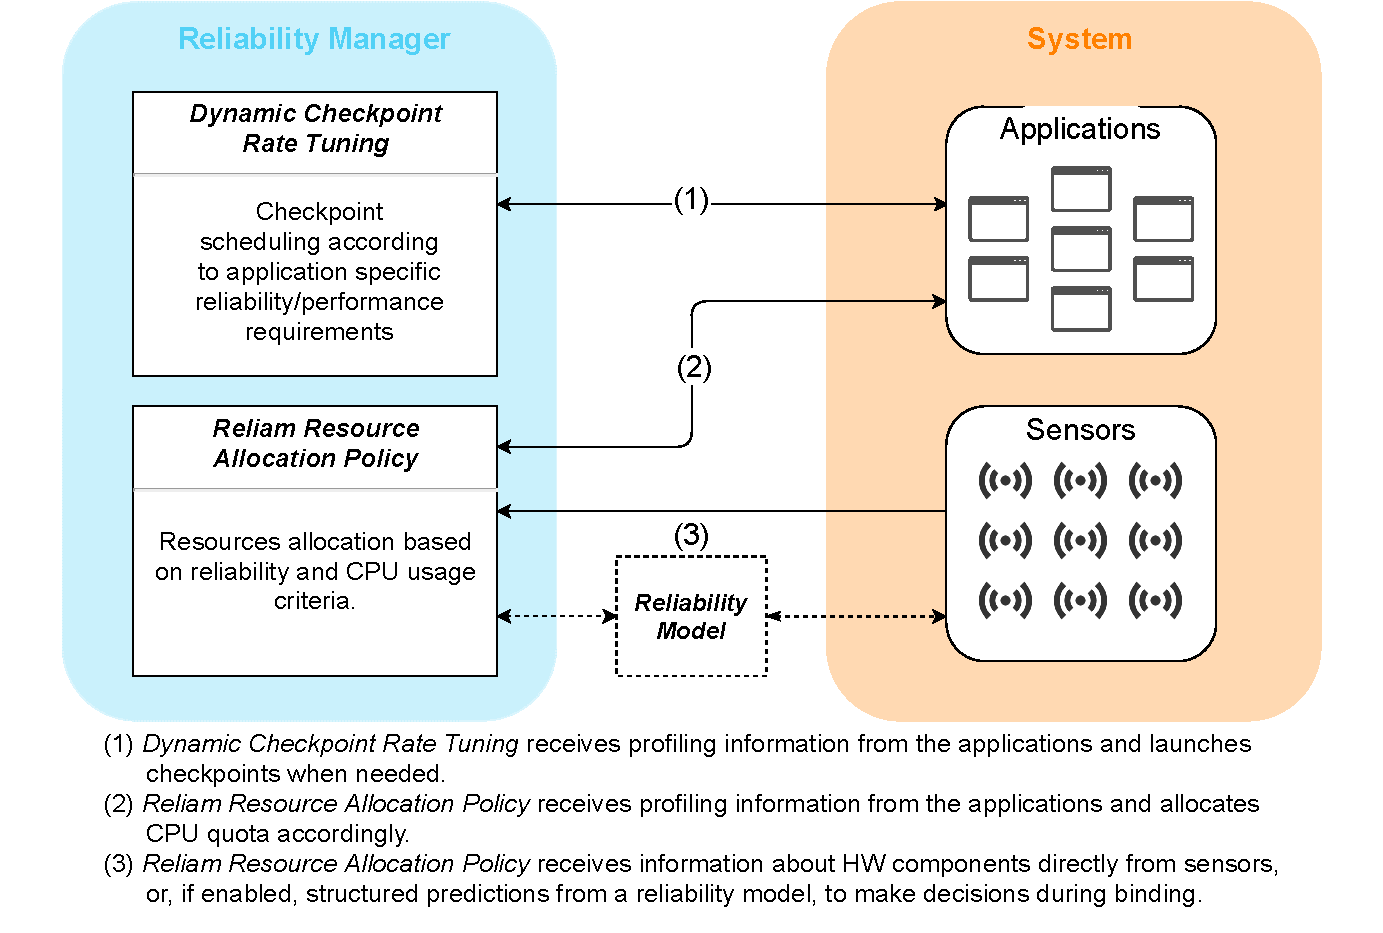
\includegraphics[width=\textwidth]{overview_thesis.pdf}
    \caption{Overview of the proposed work.}
    \label{fig:overviewth}
\end{figure}

The presented solution consists of two main components, the \emph{Dynamic Checkpoint Rate Tuning} and the \emph{Reliam Resource Allocation Policy}, which jointly contribute to achieve the above mentioned objective from different perspectives. An overview of the work, which will be deeply examined next in this chapter, is provided by Figure~\ref{fig:overviewth}.
The work proposed by this thesis is designed and implemented to be integrated both in the \emph{Barbeque Run-Time Resource Manager}, upon which an overview will be provided in the next paragraph.

\subsection{The Barbeque Run-Time Resource Manager}
\begin{figure}[t]
    \centering
    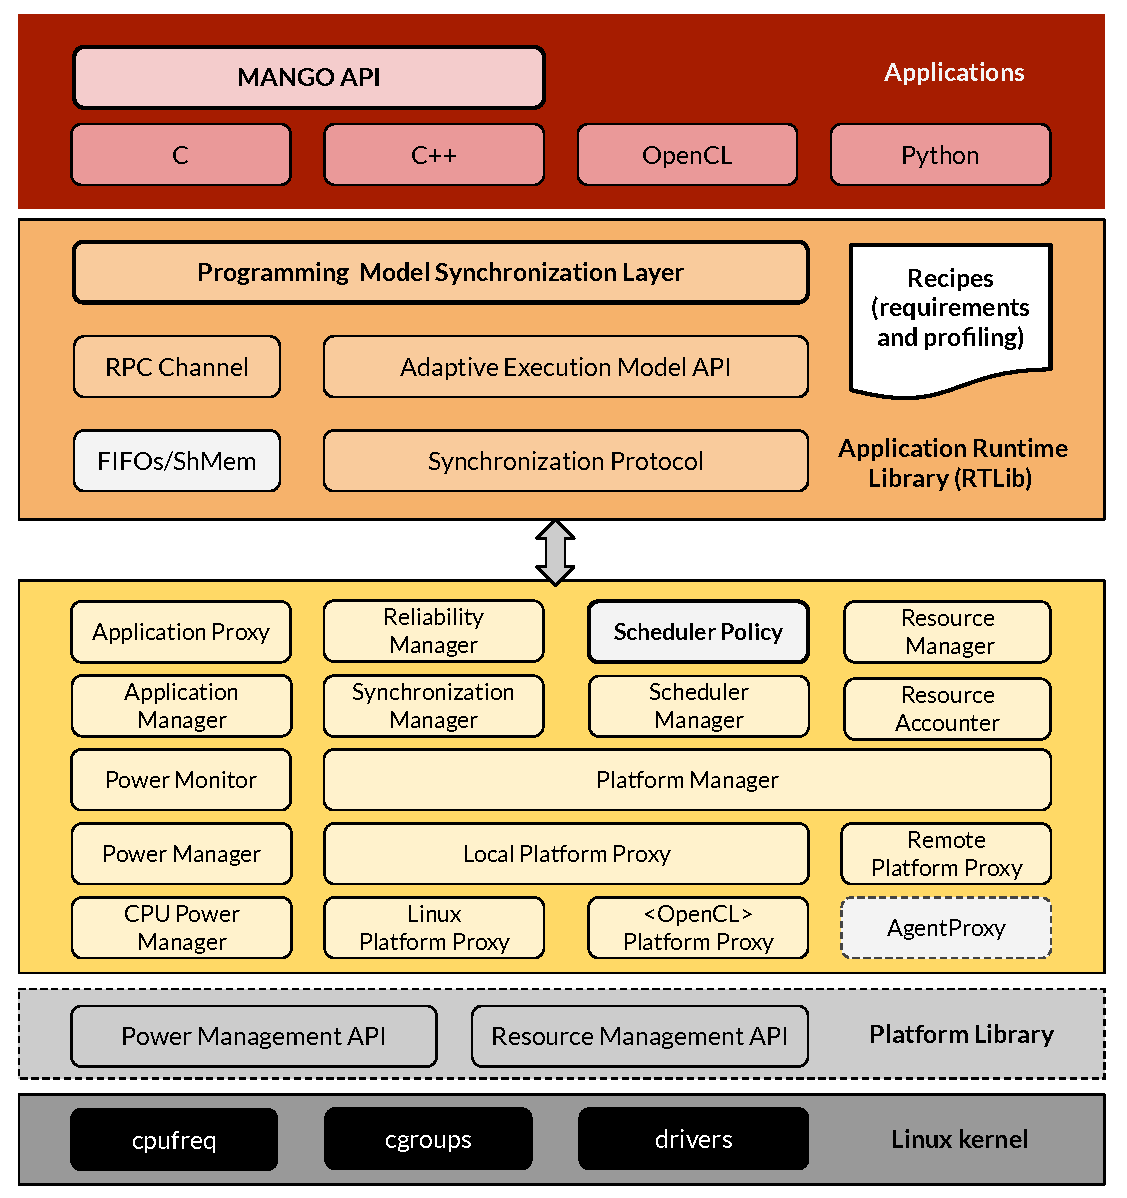
\includegraphics[width=0.8\textwidth]{bosp_architecture.pdf}
    \caption{Layer view of the BarbequeRTRM architecture.}
    \label{fig:bosp_arch}
\end{figure}
The Barbeque Run-Time Resource Manager (BarbequeRTRM) \cite{6322885} is a modular and extensible run-time resource manager that transparently manages the allocation of computing resources to multiple concurrent applications \cite{barbequertrm}. Its modular design facilitates the developer in the implementation and integration of resource allocation policies tailored to the need of each specific hardware configuration and use-case. As Figure~\ref{fig:bosp_arch} shows, the BarbequeRTRM is composed by various manager modules that provide the user with a wide range of information regarding applications, resources and optimization goals, which can be taken as input and tuned by the policy.
\begin{figure}[t]
    \centering
    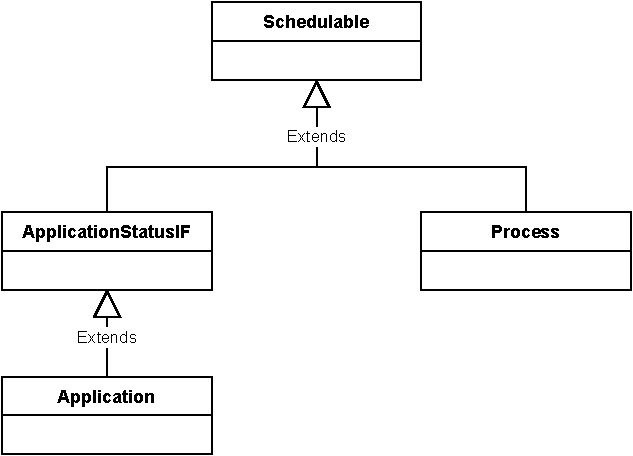
\includegraphics[width=0.8\textwidth]{uml_proc.pdf}
    \caption{Skeleton of the UML class diagram of the extensions of the class Schedulable in BarbequeRTRM.}
    \label{fig:umlproc}
\end{figure}

The framework is designed to manage the execution of generic processes, as well as integrated applications. This support is provided through the presence of a library called \verb|bbque_rtlib|, which defines a programming model called \emph{Adaptive Execution Model}, characterizing, the integrated applications. It consists in a managed execution flow in which application and Resource Manager communicate. Such interaction provides the application with a higher degree of awareness of the system, hence, the possibility to observe its own run time performance and throughput, as well as to adapt to the status of the hardware that it runs on. Conversely, it also enables the Resource Manager to assign resources taking into account the status of the system and the application requirements \cite{Zanella2019RunTimeMM}. 

The descriptors of both integrated and not-integrated applications are defined in the class \verb|Schedulable|, which stores any kind of information regarding the execution which it is instance of. Among other things, it keeps track of the process ID of the application, the state of the execution, the locality and the current resource assignment. On one hand, \verb|Schedulable| is extended by the abstract class \verb|ApplicationStatusIF| which defines an interface to query run-time information, inherited by the class \verb Application \, containing the descriptors of the integrated application. On the other hand, it is extended by the class \verb|Process|, defined to instantiate descriptors of generic processes. The above mentioned structure is shown in Figure~\ref{fig:umlproc}.

For the sake of simplicity, from now on, the terms \emph{application} and \emph{process} will be used interchangeably, since all of the features of this work have been designed and implemented for both types of workload.

\subsubsection{Hardware reliability support}
\label{sec:periodicchk}
The BarbequeRTRM is provided with a hardware reliability support based on a Periodic Checkpoint Mechanism, finalized by \emph{Checkpoint/Restore In Userspace (CRIU)}, a software tool running on Linux Operating System, as already mentioned in {\hyperref[sec:criu]{Section~\ref{sec:criu}}}. The checkpointing routine is initiated by the Reliability Manager. The function \verb|PeriodicCheckpointTask()| is called by a thread spawned at the launching of the platform and it periodically iterates over the running integrated application and managed processes, sequentially submitting them to the checkpointing procedure, without any kind of consideration of the status of the system and/or possible application requirements. To make this happen, the function \verb|Dump()| of the same module is called.  In this function, the interaction between the Reliability Manager and the Platform Manager modules takes place. Once the latter receives the checkpoint request from the former, it forwards it to the local or remote proxy able to carry out the dumping. In the case of the Local Platform Proxy, the implementations of the various \verb|Dump()| functions exposed by the Platform Proxy are called. Those proxy are, in fact, responsible of the actuation of the decisions made by the Resource Manager regarding each resource managed by the  BarbequeRTRM (CPU, NVIDIA GPU, custom accelerators, etc.) in the local node. Finally, CRIU provides to the deletion of the previous dump, if any, and to the generation of the current image, storing it in the directory specified in the configuration file of the framework.

Two limitations emerge from the current implementation:

\begin{description}
    \item [{\parbox[t]{\textwidth}{The checkpoint routine is completely unaware of the possible diversity of the running applications:}}] \hfill \\The only requirement which need to be to satisfied to proceed to the checkpointing routine is the expiration of the time period, without any kind of awareness regarding the time required by the checkpoint dump and, consequently, of the execution time left between two consecutive checkpoints of the same application. This mechanism is extended by the \emph{Dynamic Checkpoint Rate Tuning} component of this work in order to meet the reliability/performance requirements of each specific application.
    \item [{\parbox[t]{\textwidth}{The overwriting of the previous stored image results in costs in terms of reliability:}}]\hfill\\ In case of failure of the checkpoint procedure, not only the application pays the cost of the checkpoint overhead, but also has no backup until the next checkpoint, since the the previous image has been deleted. Moreover, it might happen that, even without the presence of such failure, the last checkpoint contains incorrect computation, due, for instance, to Silent Data Corruption. Also in this case, the possibility to restart from an earlier checkpoint might prevent the re-execution of all the application code. Also this weakness is taken into consideration by the proposed solution.
\end{description}

\section{Dynamic Checkpoint Rate Tuning}
\label{sec:dcrt}
The Dynamic Checkpoint Rate Tuning is one of the two main pillars of the proposed work. It takes place in the Reliability Manager module of the BarbequeRTRM and extends the already existing hardware reliability support, adding a level of application awareness to the Periodic Checkpoint Mechanism, analyzed in {\hyperref[sec:periodicchk]{Section~\ref{sec:periodicchk}}}.

\subsection{Design}
As previously anticipated, the simplicity of a periodic checkpointing algorithm is paid in terms of specificity with respect to the performance and reliability requirements of the considered application. In the case of a system in which more than one program is executing, it is reasonable to expect that, depending on the carried out functionality, each of them has different timing needs. For instance, one can think of a time critical application: if not properly tuned, the overhead produced by the checkpointing routine might cause a timing failure, an event that would highly compromise the delivered service. Conversely, in the case of a long-lasting execution application the need of a minimum overhead might be of secondary importance with respect to the need of a recent checkpoint to restart from in the event of a failure. The idea behind the Dynamic Checkpoint Rate Tuning is to adapt to both circumstances, providing the possibility to specify an upper bound on the checkpointing overhead, independently for each application. In BarbequeRTRM, this purpose is achieved by extending the Reliability Manager with a new task, carried out by the function \verb|DynamicCheckpointTask()|, called by a suitable thread at the launch of the platform, substituting the already existing \verb|PeriodicCheckpointTask()|. 

The above mentioned task must compute the following steps:
\begin{enumerate}[label={\arabic*)}]
    \item Select the next-in-list running application;
    \item Estimate the overhead that the checkpoint would bring to the execution if it were performed in that point in time;
    \item Compare the estimated overhead with the upper bound specified for the application;
    \item If the former is lower than the latter, the checkpointing routine is launched;
    \item Update checkpoint latencies of the application
    \item Go back to 1).
\end{enumerate}
As mentioned in {\hyperref[sec:periodicchk]{Section~\ref{sec:periodicchk}}}, from the reliability viewpoint, also the availability of only one saved image per time is a flaw of the current version of BarbequeRTRM: in the event of a failure in the dumping procedure, the running application is left without a useful checkpoint until the next dump is scheduled. To avoid the lack of reliability generated by this problem, a further modification has been introduced in the framework, in order to make it able to save more than one checkpoint. The extension proposed by this thesis work allows the possibility of specifying, in the configuration file, a destination folder in which a suitable number of consequent dumps are going to be stored, in order to improve the availability of a backup plan in the occurrence of failures during the execution of the application.

In the next paragraph, how the above mentioned changes have been implemented in BarbequeRTRM will be explained in details.

\subsection{Implementation}
\begin{figure}[t]
    \centering
    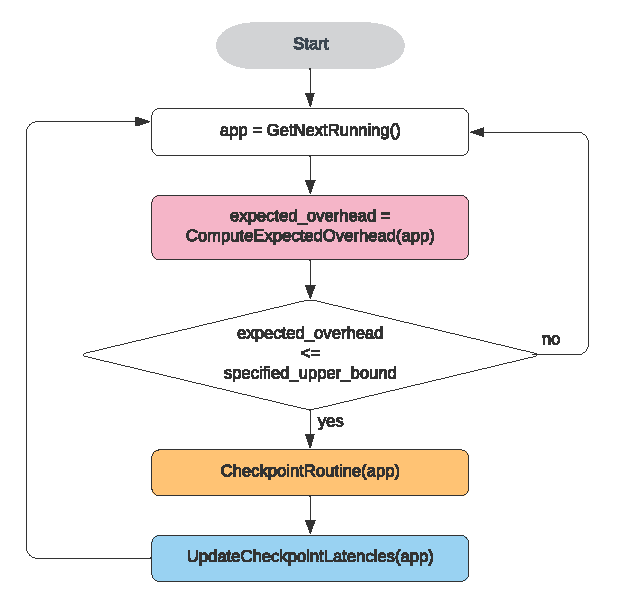
\includegraphics[width=0.6\textwidth]{dyn_chk_flow.pdf}
    \caption{Dynamic Checkpoint Rate Tuning algorithm.}
    \label{fig:dynchk}
\end{figure}
The steps followed by the Dynamic Checkpoint Rate Tuning algorithm, implemented in the function \verb DynamicCheckpointTask() \ of the Reliability Manager module, are summarized in the flowchart in Figure~\ref{fig:dynchk}, whose main basic blocks are going to be analyzed in the following sections.

\subsubsection{Computation of the expected overhead}

Given a running application, the first step of the algorithm is to compute the expected overhead a checkpoint would bring to the execution at that given point in time. 

The estimate of the checkpoint latency is given by the arithmetic mean of the previous completed dumps, stored as an attribute of the class \verb Schedulable . For each invocation of the algorithm, the expected overhead is computed considering the ratio between the cumulative amount of time spent performing checkpoints and the total time elapsed since the start of the application, in order to diminish the impact of the variance on the overhead. More specifically, the followed procedure is presented in pseudo code in Algorithm~\ref{alg:chk_overhead}.
\begin{algorithm}
    \SetKwInput{KwInput}{Input}                % Set the Input
    \SetKwInput{KwOutput}{Output}              % set the Output
    \DontPrintSemicolon
    \BlankLine
    \KwInput{Application descriptor \emph{app}}
    \KwOutput{Estimated checkpoint overhead}
    %\BlankLine
    \algrule
% Set Function Names
    \SetKwFunction{Func}{ComputeExpectedCheckpointOverhead}
% Write Function with word ``Def''
  \SetKwProg{Fn}{Def}{:}{}
  \Fn{\Func{$app$}}{
  \BlankLine
        mean\_chk\_time = app$\rightarrow$GetCheckpointLatencyMean()\;
        elapsed\_time = app$\rightarrow$GetElapsedTimeSinceStart()\;
        total\_time = elapsed\_time + expected\_chk\_time\;
        nr\_completed\_chk = app$\rightarrow$GetNrPerformedCheckpoints()\;
        sum\_chk\_time = (nr\_completed\_chk +1) * mean\_chk\_time\;
        expected\_chk\_overhead = sum\_chk\_time/total\_time\;}
        \BlankLine
        \KwRet expected\_chk\_overhead\;
    \BlankLine
   \caption{Estimation of checkpoint overhead algorithm.}
   \label{alg:chk_overhead}
\end{algorithm}


\subsubsection{Checkpoint Routine and Checkpoint Latencies Updating}
\label{sec:chkroutine}
Once computed the expected checkpoint overhead, it must be compared to the upper bound specified for considered application: if the former is not greater than the latter, the checkpoint routine starts. The control flow of the checkpoint routine is summarized in Figure~\ref{fig:chk_routine}. 

\begin{figure}[t]
    \centering
    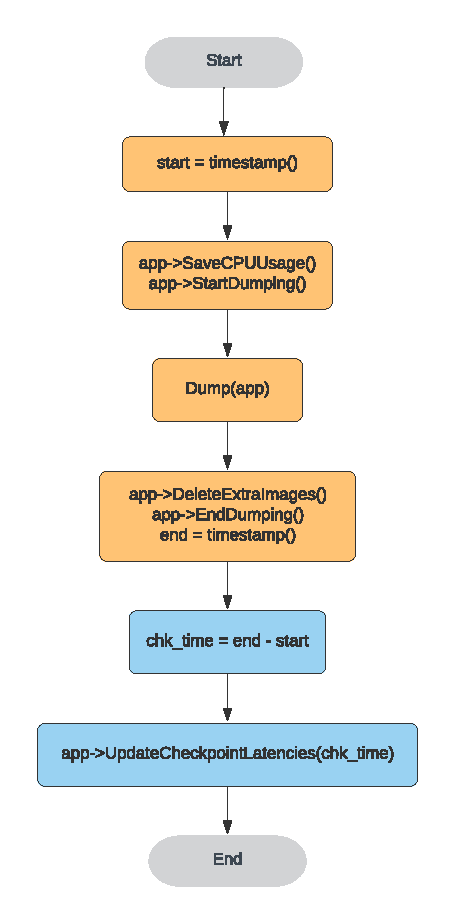
\includegraphics[width=0.5\textwidth]{chk_routine.pdf}
    \caption{Checkpoint Routine and Checkpoint Latencies Updating flowchart.}
    \label{fig:chk_routine}
\end{figure}
As a first step, the present timestamp is stored in order to keep track of the duration of the procedure. Secondarily, the current CPU usage of the application is stored and the application Boolean attribute \verb is_dumping \ is set through the member function \verb StartDumping() \footnote{A definition of \emph{CPU usage} and the motivations behind the need of this basic block will be provided in {\hyperref[sec:reliam]{Section~\ref{sec:reliam}}}.}.

After these preliminary steps, the generation of the image is performed as it was in the already existent hardware reliability support (see {\hyperref[sec:periodicchk]{Section~\ref{sec:periodicchk}}}). Differently from before, in this procedure, the deletion of the previous generated images takes place only if the number of currently saved dumps exceeds the one specified in the configuration of the framework.

The last step of the checkpoint routine is to reset the Boolean attribute of the application \verb is_dumping \ and to catch the ending timestamp.

Finally, the checkpoint latencies of the application are updated.

\section{Reliam Resource Allocation Policy}
\label{sec:reliam}
In the previous section, we discussed about the Dynamic Checkpoint Rate Tuning, the first component of this work, this section will, instead, focus on the Reliam Resource Allocation Policy. While the former was designed and implemented as a fault tolerance mechanism, i.e. to properly \emph{react} to an already occurred failure, in order to minimize its impact on the system, the latter has been conceived to \emph{proactively} improve the reliability of the hardware components.

\begin{figure}[t]
    \centering
    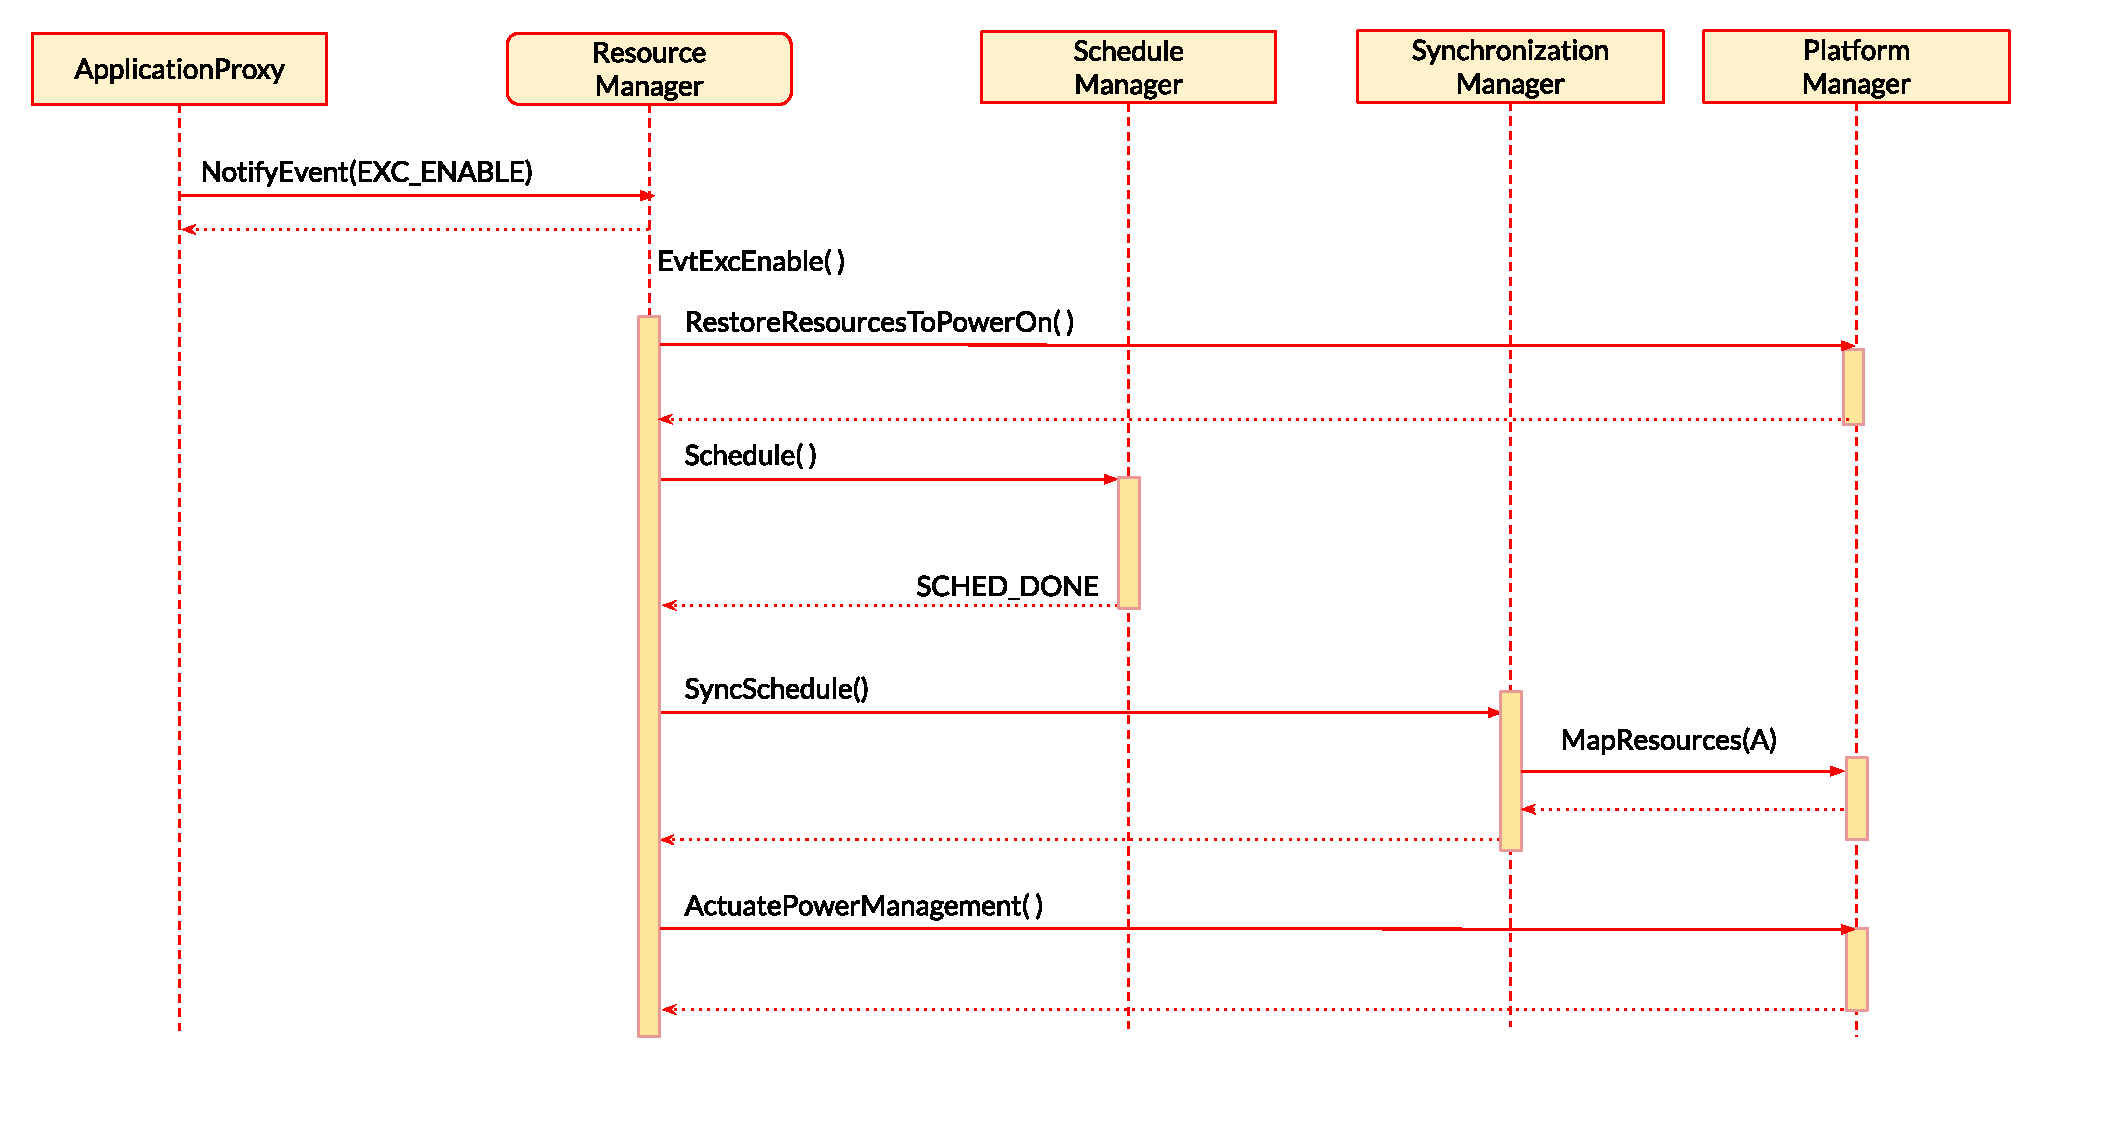
\includegraphics[width=0.95\textwidth]{bosp_flow.pdf}
    \caption{Resource assignment flow of the BarbequeRTRM.}
    \label{fig:bosp_flow}
\end{figure}

The purpose of the Reliam Resource Allocation Policy is to assign computational resources minimizing CPU usage and aging, and it is integrated as a plugin of the BarbequeRTRM.
Figure~\ref{fig:bosp_flow} summarizes the resource assignment flow of the above mentioned framework, focusing on the interaction between the main modules involved in the implementation of a generic resource allocation policy: the component discussed in this Section lies in the scheduling management part and its entry point correspond to the function \verb|Schedule()|. This function starts the execution of the allocation policy specified in the configuration phase, whose plugin is loaded when the Resource Manager is launched.

\subsection{Design}
\label{sec:poldesign}
Reliam is a resource allocation policy that must be launched on a periodical basis, whose main objective is to prevent the wear out of the computing resources and, consequently, to slow down their aging. Aside from the reliability matter, we designed a modified version of Proportional Integral Derivative (PID) controller and we implemented it to adapt the CPU quota allocation to the need of each application. This approach allowed us to reach the minimization of the CPU utilization and, consequently, better global performances, especially in the case of parallel executions. Before going into the details of the design, some definition will be firstly provided in order to guarantee the necessary background of knowledge for the reader.

\begin{description}
\item[CPU quota.]
CPU \emph{quota} is defined as the percentage, in terms of time, of CPU resources (available or allocated) where the total amount is expressed as:
\[total\_cpu\_quota = total\_nr\_cpu\_cores * 100\]
\item[CPU usage.]
Given a resource allocation to an application, we define as CPU \emph{usage} the CPU quota effectively exploited during the execution. For each application, CPU usage never exceeds the allocated CPU quota.
\item[PID controller.]
\begin{figure}[t]
    \centering
    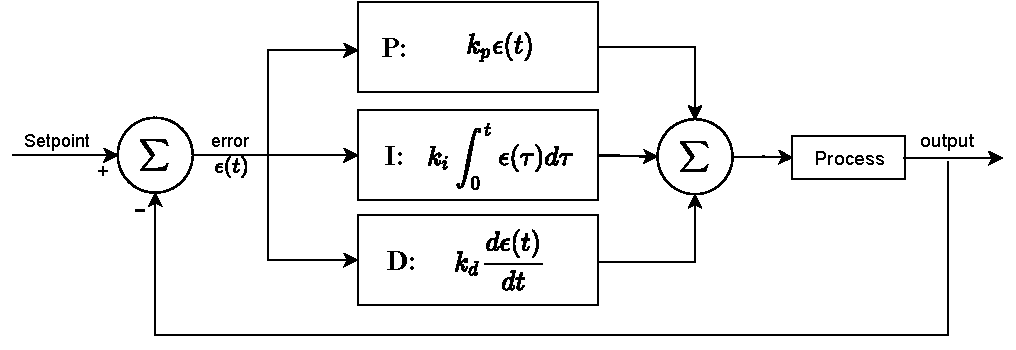
\includegraphics[width=\textwidth]{pid.pdf}
    \caption{PID controller block diagram.}
    \label{fig:pid}
\end{figure}
A PID controller is a control loop mechanism employing feedback to make the output converge to a set point, using Proportional, Integral and Derivative contributions weighted by coefficients, respectively $k_{p}$, $k_{i}$ and $k_{d}$, as shown by the block diagram in Figure~\ref{fig:pid}.

\item[Dark Silicon.]
With the end of Dennard scaling, as well as single-core scaling, also multi-core scaling is going to be constrained, due to the power limitations of the future designs, which will reduce the usable chip fraction \cite{10.1145/2024723.2000108}.
\emph{Dark Silicon} is the practice of turning off a number of cores in a chip in order to satisfy energy and thermal constraints. 
\item[Process Freezing.]
Process \emph{freezing} is a temporary and controllable pause state in the execution of a process, which will be able to resume its work after being \emph{thawed}.
\item[Process Thawing.] 
We define as process \emph{thawing} the reverse operation of freezing, after which an application is able to resume its execution.
\end{description}
\begin{figure}[t]
    \centering
    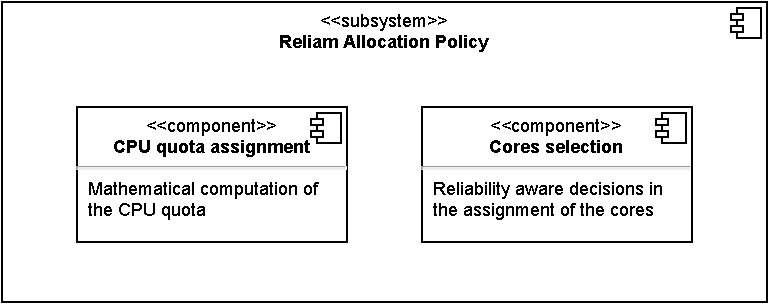
\includegraphics[width=0.8\textwidth]{comp_reliam.pdf}
    \caption{Reliam Resource Allocation Policy design components.}
    \label{fig:reliam_design}
\end{figure}

Reliam Resource Allocation Policy assigns to each application a modified version of a PID controller, in order to periodically compute the CPU quota to allocate, such that, at each invocation, it will be closer to the effective CPU usage of the application at issue. Once all CPU quotas are defined, the selection of the cores, based upon reliability criteria, is performed. The main components of the design of the policy are summarized in Figure~\ref{fig:reliam_design} and will be analyzed in depth in the next paragraphs.

\subsubsection{Computation of the CPU quota}
To better understand the rationale behind the logic of Reliam Allocation Policy 
We ideally define the PID controller variables as follows:
\begin{enumerate}[label=-]
    \item Control variable: $cv$
    \item Process variable: $\Delta$
    \item Setpoint: $\overline{\Delta}$
    \item Error: $\epsilon$
\end{enumerate}
such that:
\begin{enumerate}[label=]
    \item $cv = k_{p}*\epsilon_r + k_{i}*\sum_{k\in R}\epsilon_{k} + k_d*(\epsilon_{r}-\epsilon_{r-1})$
    \item $\Delta = CPU_{A} - CPU_{U}$
    \item $\epsilon_r = \overline{\Delta} - \Delta$
\end{enumerate}
where, considering numbered invocations of the policy, $\epsilon_r$ is the error observed at invocation $r$, while $CPU_{A}$ and $CPU_{U}$ are, respectively, the CPU quota assigned and the CPU usage of the application.

In the proposed work, we brought one fundamental change to the PID controller model in order to better fit the adaptive resource allocation problem. We decided to set to zero integral and derivative contributions in the case of \(\epsilon(t)=0\), i.e. every time the output matches the set point, avoiding pointless fluctuations of the control variable.
Considering this change in the computation of the control variable, the final ideal model is defined as follows:

\begin{flalign*}
    \renewcommand{\arraystretch}{3}
    \begin{array}{ll}
        cv &= 
            \begin{cases}
        	    k_{p}*\epsilon_r + k_{i}*\sum_{k\in R}\epsilon_{k} + k_d*(\epsilon_{r}-\epsilon_{r-1}) & \mbox{if } \epsilon\neq 0 \\
        	    0 & \mbox{otherwise}
    	    \end{cases}\\
        \Delta &= CPU_{A} - CPU_{U} \\
    	\epsilon_r &= \overline{\Delta} - \Delta
	\end{array}
\end{flalign*}

Once defined the ideal model, we need to introduce slight changes to the process variable $\Delta$ and the computation of the error $\epsilon$ for the sake of the applicability in a real scenario.

\begin{description}
\item[Process variable: $\Delta$.]
Consider the $r^{th}$ invocation of the policy with $r>1$.
Given a CPU quota allocation to an application, if, in the previous invocation, the CPU quota has exceeded the observed CPU usage, it is reasonable to infer that a lesser assignment can be performed. The process variable $\Delta$ is computed as:
\begin{align*}
    \Delta = CPU_{A} - CPU_{U}
\end{align*}
Conversely, $CPU_{A} == CPU_{U}$ means that the application saturated all the assigned resources, thus it might use more of them if available. As already mentioned, the following inequality always applies: 
\begin{align*}
    CPU_{U} \leq CPU_{A}
\end{align*}
Since, in this scenario, we are not able to infer the CPU usage the application would have shown if a larger CPU quota had been assigned to it, we assign to $\Delta$ a negative constant:
\begin{align*}
    \Delta = \Delta_{NEG}
\end{align*}
This modification to the ideal $\Delta$ allows us to a more balanced use of the controller, which, otherwise, would have properly worked only with positive values of $\Delta$.
\item[Error: $\epsilon$.]
\begin{figure}[t]
    \centering
    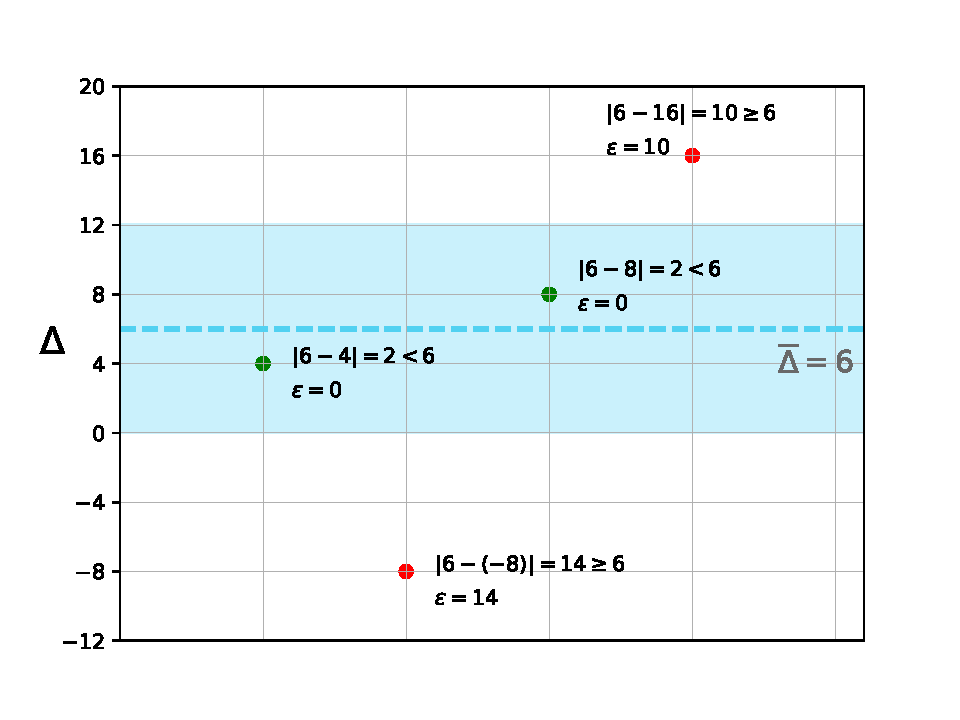
\includegraphics[width=0.8\textwidth]{delta.pdf}\vspace{-1.15em}
    \caption{Graphical explanation of the computation of the error in the real model of the modified PID Controller. The blue area corresponds to the values of $\Delta$ such that $\epsilon=0$.}
    \label{fig:delta}
\end{figure}
During its execution, it is reasonable that an application maintains the same CPU usage, net of some small variation. In order to avoid a new computation of the quota if, in two consecutive invocations, the observed CPU usage is similar but not equal, we relaxed the computation of $\epsilon$ in order to be 0 if $\Delta$ is \emph{close enough} to $\overline{\Delta}$, such that if:
\begin{flalign*}
    |\overline{\Delta}-\Delta| \leq \overline{\Delta}
\end{flalign*}
given that:
\begin{flalign*}
    |\overline{\Delta}-\Delta_{NEG}| \geq \overline{\Delta} 
\end{flalign*}
the error $\epsilon$ remains equal to zero.
\end{description}
Changes above considered, we can finally define the real model as:
\begin{enumerate}[label=-]
    \item Control variable: $cv$
    \item Process variable: $\Delta$
    \item Setpoint: $\overline{\Delta}$
    \item Error: $\epsilon$
\end{enumerate}
where:
\begin{align*}
    \renewcommand{\arraystretch}{3}
    \begin{array}{ll}
        cv &= 
        \begin{cases}
                k_{p}*\epsilon_r + k_{i}*\sum_{k\in R}\epsilon_{k} + k_d*(\epsilon_{r}-\epsilon_{r-1}) & \qquad \mbox{if } \epsilon\neq 0 \\
        	    0 & \qquad\mbox{otherwise} 
        \end{cases}\\
        \Delta &= 
            \begin{cases}
        	    CPU_{A} - CPU_{U} \hfill& \qquad \mbox{if } CPU_{A} > CPU_{U} \\
        	    \Delta_{NEG} &\qquad \text{otherwise}
    	    \end{cases}\\
    	    \epsilon &=
    	    \begin{cases}
        	    \overline{\Delta} - \Delta &\qquad\mbox{if } |\overline{\Delta}-\Delta| \geq \overline{\Delta}\mbox{}\\
        	    0 &\qquad \mbox{otherwise}
    	    \end{cases}
	\end{array}
\end{align*}


A graphical explanation of the computation of the error is provided in Figure~\ref{fig:delta}. In the example, $\overline{\Delta}=6$, hence, the values of $\Delta$ marked in green produce $\epsilon=0$, while $\epsilon=\overline{\Delta}-\Delta$ for the ones colored in red.

\subsubsection{CPU cores selection and reliability monitor}
\label{sec:corsel}
In the previous paragraph, we defined the model used to compute the CPU quota assigned by the policy to the applications, in this one, we will provide details about the selection of the processing elements that are supposed to provide such CPU quota.

The idea behind the designed selection mechanism is to emulate at software level the effect of Dark Silicon, in order to keep the temperature of the system components in a safe operating range. The above mentioned goal is achieved allocating the CPU cores in a sequential fashion\cprotect\footnote{BarbequeRTRM provides two policies of CPU quota partitioning:
\begin{itemize}
    \item SEQUENTIAL: a new core is bound to the application only if all the CPU quota associated to the previous one has been allocated;
    \item BALANCED: each available core equally contributes to the handling of the request.
\end{itemize}}, i.e. saturating the quota of each bound core, in ascending order of temperature, before allocating a new one. In this way we obtain that, in the case in which not all computational resources available in the system are needed, warmer cores are the ones that remain idled. Moreover, in all circumstances, all the processing elements exceeding their safety critical temperature are forced to idle. The policy is also entrusted with the ability of freezing applications classified as \emph{critical} with respect to the reliability of the system. More specifically, an application will be frozen if all the processing element bound to it with quota 100 are exceeding their safety critical temperature. In this way, the idling of those cores will impact only on the performance of that specific application and not on the entire system. Since, at the time of writing, modern Intel CPUs apply \emph{Dynamic Voltage and Frequency Scaling (DVFS)} at hardware/firmware level, we do not have the possibility to directly resort to such technique at software level. Nonetheless, its contribution is transparently added to the effectiveness of our solution by the design of the processing units.

Furthermore, the flexibility of the policy allows the possibility to consider more than one reliability input. Core temperature measurement can be combined with more comprehensive reliability profiling data, if compatible monitoring tools or interfaces are integrated with the Reliam Resource Allocation Policy. At the time of writing, BarbequeRTRM is provided with a library called \verb|libhwrel| \cite{recipedel} which consists of a hardware reliability monitor able to predict the degradation of their reliability. It is composed by three main classes: \verb|Request|, which contains the requests sent by the Resource Manager to the library, \verb|Response| which contains the response to such requests, and the main class \verb|HWReliabilityMonitor| which performs the actual analysis, taking a \verb|Request| object as an input and providing a \verb|Response| object as an output. In the requests, it is possible to specify the resource type (CPU, GPU, Memory, etc.) and the technology used (ASIC, FPGA, etc.): after appropriate analysis, the library will output a number representing the probability of failure in per-mille/program-run \cite{recipedel}. If \verb|libhwrel| is linked to the policy, the ordering of the cores will be made in ascending order of their \verb|Response| output of the \verb|libhwrel|.

For the sake of generality, in the following section, the basic implementation, extracting the temperature values directly through the sensors output, will be examined.

\subsection{Implementation}
\begin{figure}[t]
    \centering
    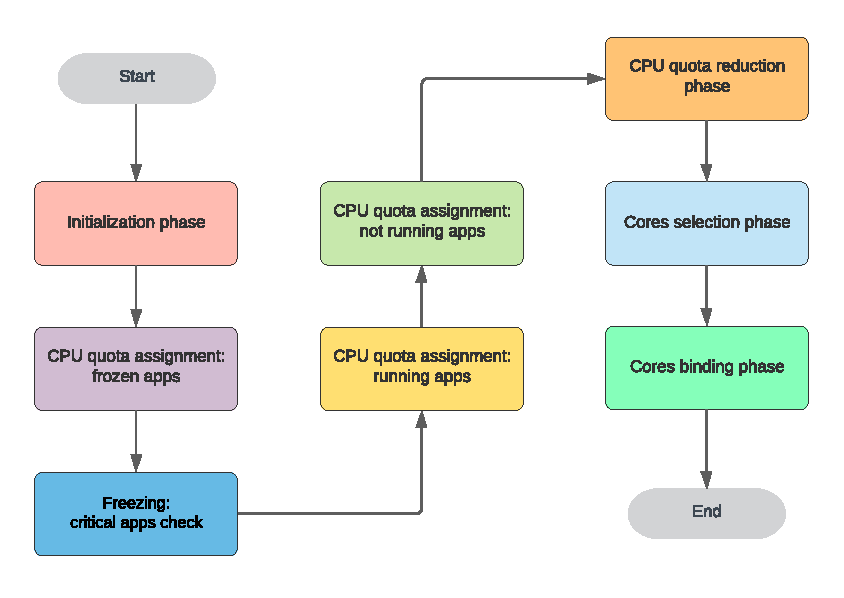
\includegraphics[width=\textwidth]{policy_flow.pdf}
    \caption{Control flow of the Reliam Resource Allocation Policy.}
    \label{fig:policyflow}
\end{figure}

Reliam Resource Allocation Policy has been implemented in the BarbequeRTRM following the sequential control flow shown in Figure~\ref{fig:policyflow}. All blocks will be independently examined in the following paragraphs, since the sequential structure of the policy allows an easily done partitioning in basic blocks. 

Before examining in depth the implementation of the policy some preliminary information is provided:
\begin{itemize}
\item The map \verb|assigned_quotas|, having as key the application descriptor descriptor and as value the its computed CPU quota is instantiated as an attribute of the class: every time a CPU quota is computed, an element is added to the map;
\item Given an application, it is always possible to retrieve its last assigned CPU quota: in this thesis, for the sake of simplicity, it will be always done through the use of the function \verb|GetPrevQuota()|;
\item Given an application, it is always possible to retrieve its CPU usage \emph{respective to the last point in time in which it was executing}: in this thesis, for the sake of simplicity, it will be always done through the use of the function \verb|GetCPUUsage()|. Considering, for instance, a resource allocation taking place right after the performing of a checkpoint, such function will return the CPU usage of the moment right before the suspension of the execution.
\item In this paper we will refer to the CPU quota assigned in the current invocation of the policy as \emph{next\_quota}, while \emph{prev\_quota} will refer to the CPU quota assigned in the invocation right before the current one.
\end{itemize}
\begin{figure}[t]
    \centering
    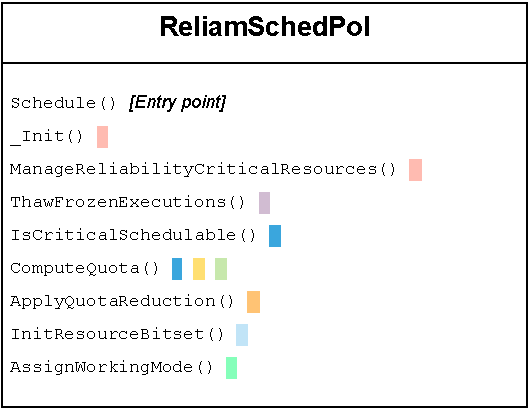
\includegraphics[width=0.6\textwidth]{reliam_uml.pdf}
    \cprotect\caption{Partial UML class diagram of the class \verb|ReliamSchedPol|.}
    \label{fig:reliamuml}
\end{figure}

In Figure~\ref{fig:reliamuml},  a partial UML class diagram of class  \verb|ReliamSchedPol|, implementing the Reliam Resource Allocation Policy, is shown: the main member functions are listed, next to the colors of the basic blocks of the flowchart in Figure~\ref{fig:policyflow} that they implement.

\subsubsection{Initialization phase}
\label{sec:init}
The initialization phase takes place in the member functions \verb _Init() \ and \verb|ManageReliabilityCriticalResources()|, directly called by \verb|Schedule()|, the entry function of the policy. During initialization, the definition of the main inputs of the policy takes place. In order to ensure the functioning of the design described in the previous section, the following attributes are initialized:

\newcommand\vitem[1][]{\SaveVerb[%
    aftersave={\item[\textnormal{\UseVerb[#1]{vsave}}]}]{vsave}}
\begin{description}
    \vitem +nr_not_running_apps:+ the number of managed applications not scheduled yet. This information is directly provided by the Application and Process Manager modules of the framework.
    \vitem +id_cpu_cores_to_idle:+ list of the id of CPU cores that are going to be forced to idle by the policy, for reliability reasons. This information is computed comparing the critical temperature of each core against the current one. Both pieces of information are fetched through the Power Manager module. 
    \vitem +nr_cpu_cores_to_idle:+ the number of CPU cores to set to idle mode for reliability reasons. It is the size of the list defined in the previous attribute.
    \vitem +nr_cpu_cores_prev_idle:+ the number of CPU cores forced to idle mode for reliability reasons in the previous invocation of the policy. Such information it is stored by the policy in the Reliability Manager at each invocation.
    \vitem +nr_cpu_cores_resumed_from_idle:+ difference in the number of cores idled between the previous and the current invocation, i.e. \verb nr_cpu_cores_prev_idle \ - \verb|nr_cpu_cores_to_idle|. 
    \vitem +available_cpu_cores:+ list containing the descriptors of all the CPU cores available in the system.
    \vitem +available_cpu_quota:+ the total CPU quota allocatable by the policy, net of the amount corresponding to the cores that are going to be idled in the current invocation. Given the number of cores available in the system \verb total_nr_cpu_cores , it is computed as:  \verb (total_nr_cpu_cores \ - \verb|nr_cpu_cores_to_idle)*100|. Every time a CPU quota is assigned to application, this variable will be decremented by such assignment to keep track of the residual availability.
\end{description}
Once all of the necessary information has been retrieved, the actual computation takes place.

\subsubsection{CPU quota assignment: frozen applications}
As mentioned in the design of the \emph{cores selection} component, it is possible for the policy to freeze a \emph{critical} application, for reliability reasons (details will be provided in the next paragraph). As a consequence of this feature, at each invocation, right after the initialization phase, the first step of the policy results in checking the necessary condition to thaw frozen executions, if any. 

\verb nr_cpu_cores_resumed_from_idle \ > 0 is the necessary condition to start the thawing process and it is checked in the member function  \verb|ThawFrozenExecutions()|.

More specifically, the policy iterates over the frozen applications, thawing them and assigning as much CPU quota as possible, considering as upper bound the smaller value between the last CPU quota assigned before it was frozen and \verb|nr_cpu_cores_resumed_from_idle*100|.
Algorithm~\ref{alg:thaw} shows the exact procedure followed by the first computational step of the policy. 
\begin{algorithm}[t]
    \SetKwInput{KwInput}{Input}                % Set the Input
    \SetKwInput{KwOutput}{Output}              % set the Output
    \DontPrintSemicolon
    \BlankLine
    \KwInput{\FuncSty{available\_cpu\_quota, nr\_cpu\_cores\_resumed\_from\_idle}}
 %   \KwInput{\FuncSty{nr\_cpu\_cores\_resumed\_from\_idle}}
    \KwOutput{None}
    %\BlankLine
    \algrule
% Set Function Names
    \SetKwFunction{Func}{ThawFrozenExecutions}
% Write Function with word ``Def''
  \SetKwProg{Fn}{Def}{:}{}
  \Fn{\Func{available\_cpu\_quota,  nr\_cpu\_cores\_resumed\_from\_idle}}{
  \BlankLine
        resumed\_cores = nr\_cpu\_cores\_resumed\_from\_idle\; 
        \While{resumed\_cores > 0}
        {
            app = GetNextFrozen()\;
            prev\_quota = app$\rightarrow$GetPrevQuota()\tcp*[r]{last quota}
            \eIf{prev\_quota/100 > resumed\_quota}
            {
                 assigned\_quotas[app] = resumed\_cores*100\;
                 resumed\_cores = 0 \;
            }{
                assigned\_quotas[app] = prev\_quota\;
                resumed\_cores -= prev\_quota/100\;
            }
            available\_cpu\_quota -= assigned\_quotas[app]\;
            Thaw(app)\;
        }
    }
        \BlankLine
    \BlankLine
   \caption{Process Thawing algorithm.}
   \label{alg:thaw}
\end{algorithm}


\subsubsection{Freezing: critical applications check}
As already anticipated, the policy has been provided with the capability of freezing an application in the case it has been acknowledged as \emph{critical}. More specifically, we classify as critical each application such that, after the initialization phase, the list \verb|id_cpu_cores_to_idle| contains as elements \emph{all} the IDs of the CPU cores assigned to such application \emph{with CPU quota equal to 100}. The check at issue and is carried out by the boolean member function \verb|IsCriticalSchedulable()|, called by \verb|ComputeQuota()|. If the return value is \verb true , the latter takes care of saving the amount of the lastly assigned CPU quota, in order ensure its retrieval, in later invocations of the policy, by the procedure described in the previous paragraph. The control flow of this entire algorithm can be found in Figure~\ref{fig:freeze}.
\begin{figure}[t]
    \centering
    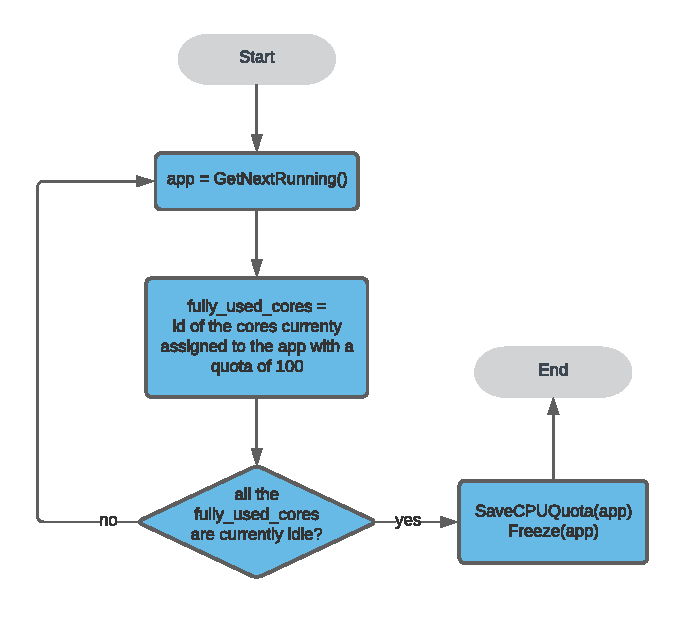
\includegraphics[width=0.9\textwidth]{check_to_freeze.pdf}
    \caption{Critical applications check.}
    \label{fig:freeze}
\end{figure}

\subsubsection{CPU quota assignment: running applications}
The basic block concerning the computation of the CPU quota to allocate for running application represents the core of the policy and consists in the implementation of the model described in the {\hyperref[sec:poldesign]{Design Section}}. The control flow of this component, for each application at issue, is described by Figure~\ref{fig:runapp}. 
\begin{figure}[t]
    \centering
    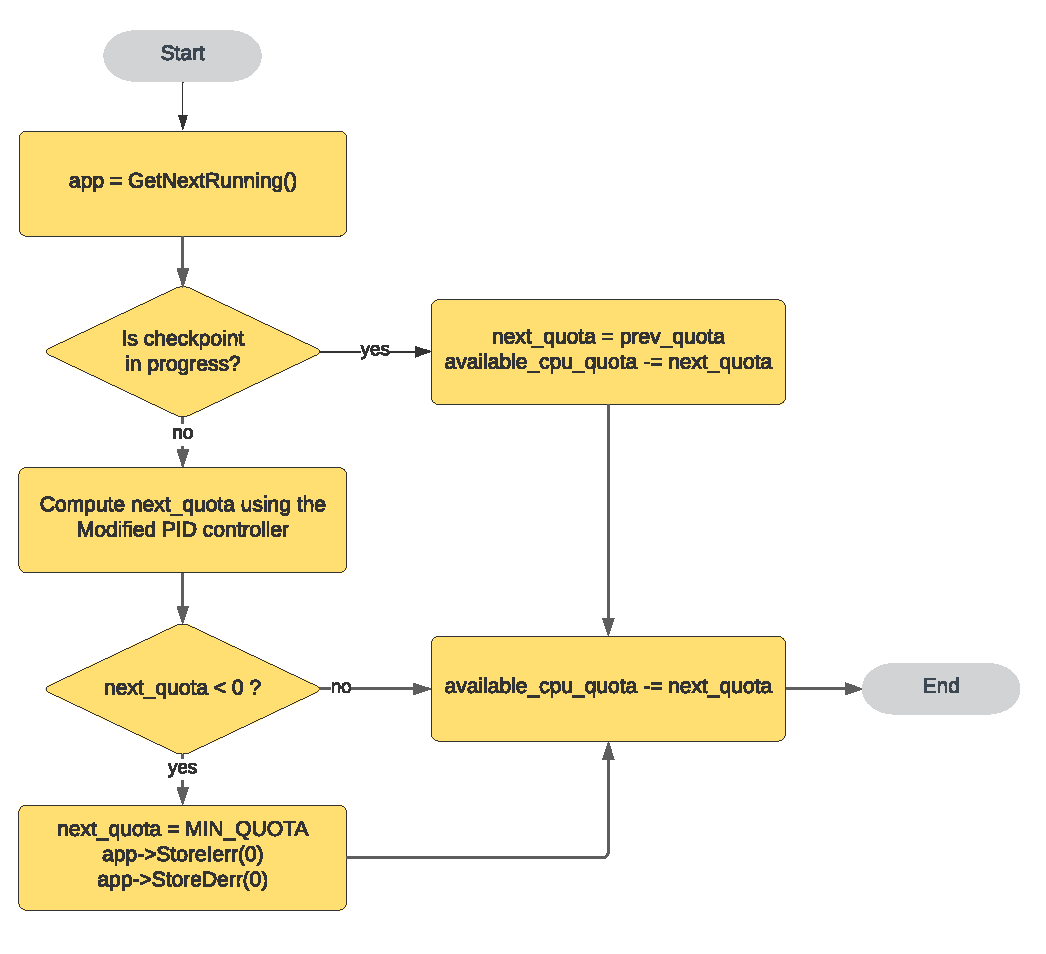
\includegraphics[width=0.8\textwidth]{running_apps.pdf}
    \caption{CPU quota assignment for running app control flow.}
    \label{fig:runapp}
\end{figure}

As shown in the above mentioned flowchart, the first step of the procedure is checking if a checkpointing of the application at issue is taking place. This check is possible thanks to the setting of the Boolean attribute of the application \verb is_dumping , carried out by the checkpointing routine previously considered in this work\footnote{See paragraph {\hyperref[sec:chkroutine]{\emph{Checkpoint Routine and Checkpoint Latencies Updating}}} of this chapter.}. If such attribute is set, i.e. the checkpointing is in progress, the policy will allocate for the application the same CPU quota lastly assigned.
Conversely, if the application is regularly executing, the Modified PID controller will compute the new CPU quota to assign. Algorithm~\ref{alg:pid} shows the pseudo-code of the procedure followed by the controller, implementing the model previously designed in this Section.

\begin{algorithm}
    \SetKwInput{KwInput}{Input}  
    \SetKwInput{KwConstant}{Constant}% Set the Input
    \SetKwInput{KwOutput}{Output}              % set the Output
    \DontPrintSemicolon
    \BlankLine
    \KwInput{Application~descriptor:~\emph{app}}
    \KwOutput{Assigned CPU quota: \emph{next\_quota}}
    \KwConstant{\ArgSty{ADMISSIBLE\_DELTA, NEG\_DELTA, Kp, Ki, Kd}}
    %\BlankLine
    \algrule
% Set Function Names
% Write Function with word ``Def''
 \nonl\emph{Modified PID Controller:}\;
\BlankLine
  {
    prev\_quota = app$\rightarrow$GetPrevQuota()\;
    cpu\_usage = app$\rightarrow$GetCPUUsage()\;
    delta = prev\_quota - cpu\_usage\;
    error = ADMISSIBLE\_DELTA/2 - delta\;
    
   
    \uIf{delta == 0 \tcp*[r]{all assigned resources have been used}}
    {
        delta = \ArgSty{NEG\_DELTA}
    }
    
    \ElseIf{ (abs(error) < ADMISSIBLE\_DELTA/2)}
        {error = 0\tcp*[r]{admissible range}
        app$\rightarrow$StoreIerr(0)\;
        app$\rightarrow$StoreDerr(0)\;}
    
    pvar = Kp*error\tcp*[r]{PROPORTIONAL CONTROLLER}

    
    ierr = error + app$\rightarrow$ierr\;
    app$\rightarrow$StoreIerr(ierr)\;
    ivar = Ki*ierr\tcp*[r]{INTEGRAL CONTROLLER}
    
   
    derr = error - app$\rightarrow$derr\; 
     app$\rightarrow$StoreDerr(derr)\;
    dvar = Kd*derr \tcp*[r]{DERIVATIVE CONTROLLER}

    cv = pvar + ivar + dvar\tcp*[r]{control variable}
    
     next\_quota = prev\_quota + cv\tcp*[r]{assigned quota}
     \KwRet{next\_quota}
  \BlankLine
        
    }
        \BlankLine
    \BlankLine
   \caption{Modified PID controller algorithm.}
   \label{alg:pid}
\end{algorithm}

Since the model is blind with respect to the fact that the allocated CPU quota must be greater than zero, a last check is needed: if the above mentioned condition is not satisfied, a \emph{minimum default value} will be allocated and the Integral and Derivative contributions reset.

\subsubsection{CPU quota assignment: not running applications}
\begin{figure}[t]
    \centering
    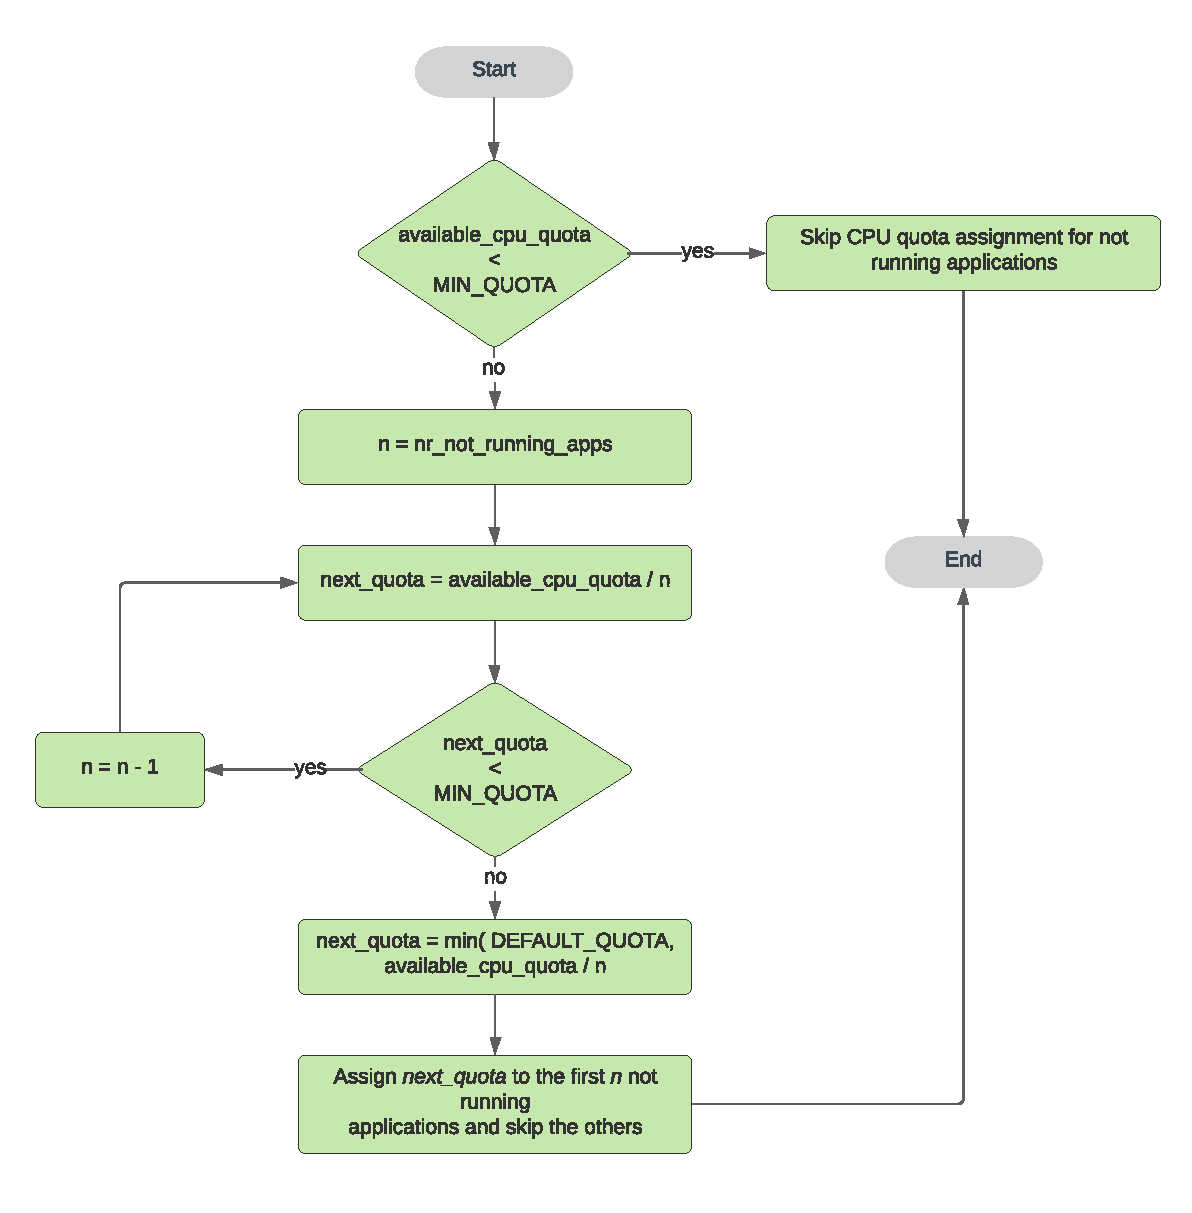
\includegraphics[width=0.9\textwidth]{not_running.pdf}
    \caption{CPU quota assignment for not running applications.}
    \label{fig:notrun}
\end{figure}
Last step of the CPU quota assignment phase of the Reliam Scheduling Policy is the computation of the quota for every application whose execution is not started yet. In this scenario we designed a \emph{fair} behaviour, i.e. a uniform CPU quota allocation among the scheduled applications. The CPU quota allocated for each application will be bounded between two constant values, \verb MIN_QUOTA \ and \verb DEFAULT_QUOTA \, depending on the \verb available_cpu_quota \ and on the number of pending applications. More specifically, it might happen that, if a fair assignment does not allow the allocation to be in the range of values mentioned above, a number of applications will not be scheduled for execution. The flowchart in Figure~\ref{fig:notrun} provides the details about how the assignment is computed for this last set of applications.
\begin{figure}[t]
    \centering
    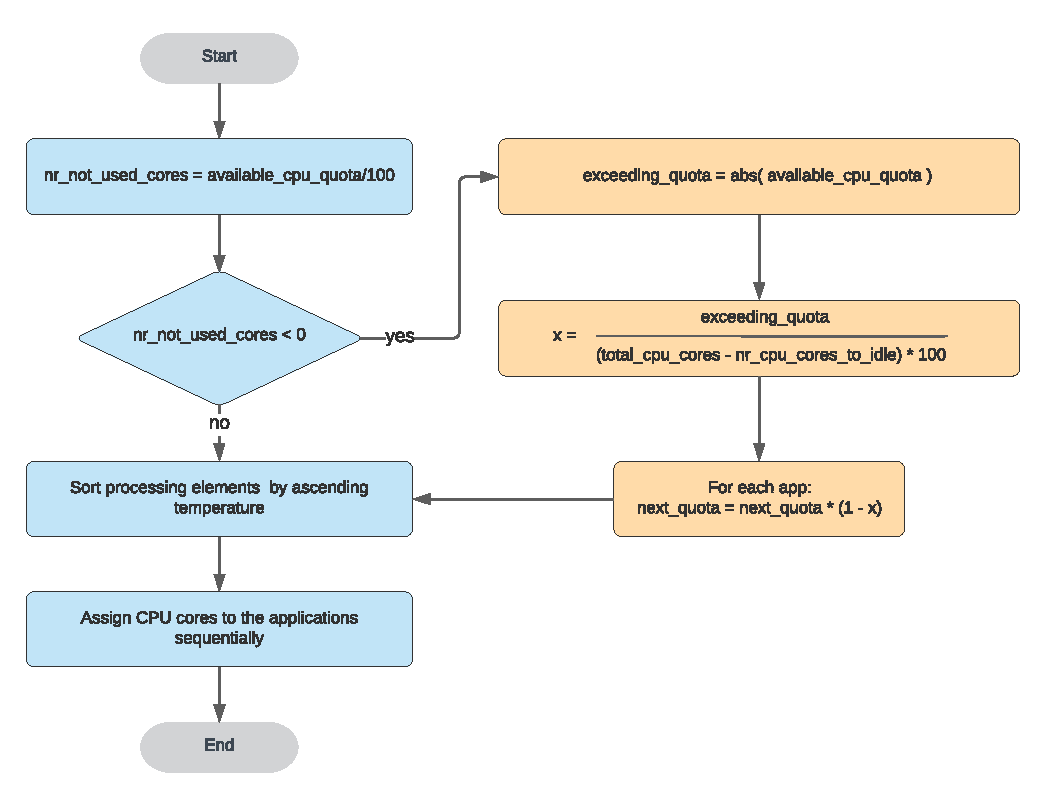
\includegraphics[width=\textwidth]{quota_red.pdf}
    \caption{Cores selection and CPU quota reduction control flow.}
    \label{fig:quotared}
\end{figure}

\subsubsection{CPU quota reduction and Core selection phases}
\label{sec:coresel}
Apart from the case of not running application, addressed by the previous paragraph, the policy allocates the CPU quota blindly with respect to the actual resources availability of the system. At each step, after being computed, the assigned CPU quota is subtracted from the variable \verb|available_cpu_quota| which, at the end of procedure, might be lower than zero. The occurrence of this event points out the fact that a CPU quota reduction is needed, since the summation of all the CPU quotas assigned by the controller is not compatible with the availability in the system, hence, it must be corrected. The CPU quota reduction has been implemented in the member function \verb|ApplyQuotaReduction()|. It computes the amount of exceeding assigned CPU quota with respect to the actually available amount as follows:
\[x = \frac{exceeding\_cpu\_quota}{(total\_nr\_cpu\_cores-nr\_cpu\_cores\_to\_idle)*100}^\text{\footnotemark}\]\cprotect\footnotetext{The denominator of this formula is the value of \verb|available_cpu_quota| at {\hyperref[sec:init]{\emph{Initialization phase}}}.}
where the numerator $exceeding\_cpu\_quota$ is computed as the absolute value of \verb|available_cpu_quota|. In the above mentioned equation, $x$ represents the ratio between the exceeding assigned CPU quota and the total allocatable amount. This ratio is used to subtract a proportional quantity of the assignment from each scheduled application, i.e. for each application, the assigned CPU quota will be reduced as follows:
\[reduced\_quota = computed\_quota * (1 - x)\]
Once, if it was needed, the CPU quota reduction phase has been completed, the selection of the cores to bind takes place. In this phase, carried out by the member function \verb|InitResourceBitset()|, a number of CPU cores is forced in idle mode by setting to zero their value in a \emph{bitset} provided by BarbequeRTRM to allow the choice of the processing elements to bind. The idled CPU cores will correspond to the ones having the highest temperature, in a number determined as:
\begin{flalign*}
nr\_idled\_cpu\_cores = max(nr\_cpu\_cores\_to\_idle,\\
nr\_cpu\_cores\_to\_idle + available\_cpu\_quota)
\end{flalign*}
where $nr\_cpu\_cores\_to\_idle$ is the value of the homonym variable defined at {\hyperref[sec:init]{\emph{Initialization phase}}}.

\subsubsection{Cores binding phase}
For each application, the binding of the CPU cores is implemented in the member function \verb|AssignWorkingMode()| and follows the the generic procedure provided by BarbequeRTRM, summarized below:
\begin{enumerate}
    \item A \verb|WorkingMode| object is instantiated;
    \item A resource requests is added, containing the generic path of the  CPU resources, the CPU quota and the way in which it must be split among the resources\cprotect\footnote{As already mentioned in the {\hyperref[sec:poldesign]{\emph{Design Section}}}, a sequential policy is used in this work.};
    \item The binding of such request to the registered resources is finalized, specifying the bitset initialized in the {\hyperref[sec:coresel]{\emph{Core selection phase}}}.
\end{enumerate}
